\uuid{AB4A}
\exo7id{7131}
\titre{exo7 7131}
\auteur{megy}
\organisation{exo7}
\datecreate{2017-02-08}
\isIndication{true}
\isCorrection{true}
\chapitre{Géométrie affine euclidienne}
\sousChapitre{Géométrie affine euclidienne du plan}
\module{Géométrie}
\niveau{L2}
\difficulte{}

\contenu{
\texte{
% joli, points cocycliques
Soit $ABC$ un triangle non rectangle et $A'$, $B'$, $C'$ les pieds des hauteurs. Montrer que les hauteurs de $ABC$ sont des bissectrices du triangle $A'B'C'$, dit \emph{triangle orthique}.
}
\indication{Utiliser les angles droits pour montrer que des points sont cocycliques, puis utiliser le théorème de l'angle inscrit.}
\reponse{
Le quadrilatère $ABA'B'$ est inscriptible dans un cercle de diamètre $[AB]$. En effet, les triangles $ABA'$ et $ABB'$ sont par définition rectangles en $A'$ et $B'$, et ont même hypoténuse $[AB]$.

De même, les quadrilatères $BCB'C'$ et $CAC'A'$ sont inscriptibles dans des cercles de diamètre $[BC]$ et $[CA]$.

\begin{center}
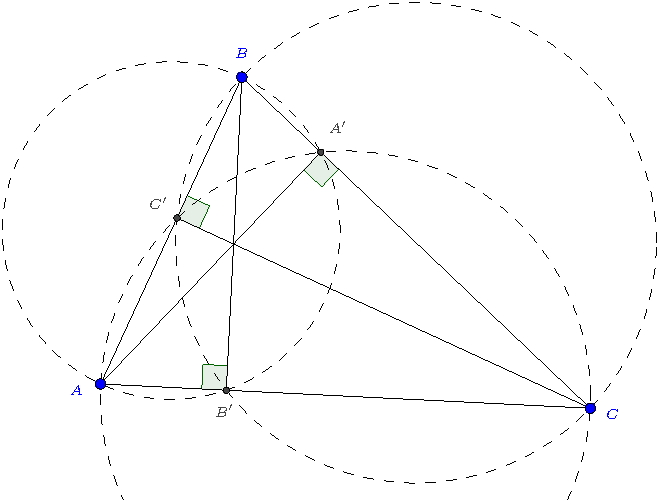
\includegraphics{../images/pdf/AB4A-1.pdf}
\end{center}

Montrons que la hauteur $(BB')$ est une bissectrice des droites $(B'C')$ et $(B'A')$. Pour cela, on montre que $(B'C',B'B)=(B'B,B'A')$.

On a :
\begin{align*}
(B'C',B'B)
&= (CC',CB) \text{ (car $BCB'C'$ est inscriptible)}\\
&= (CC',CA') \text{ (mêmes droites)}\\
&= (AC'AA') \text{ (car $ACA'C'$ est inscriptible)}\\
&= (AB,AA') \text{ (mêmes droites)}\\
&= (B'B,B'A') \text{ (car $ABA'B'$ est inscriptible)}\\
\end{align*}
}
}
